\section{Resultados e discussões}
Nesta seção são apresentados os resultados obtidos para cada algoritmo de ordenação implementado. Para cada um, é discutida sua complexidade teórica, apresentado o código-fonte correspondente e analisado o desempenho por meio de gráficos gerados com os tempos de execução coletados nas simulações.

\newpage
\subsection{Funções e macros utilizadas}
\begin{lstlisting}[language=C, caption={Funções e macros}, label={lst:macros}]
#define ARRAY_SIZE(v) sizeof(v)/sizeof(v[0])
static inline void swap(int *a, int *b) { if(a!=b) { (*a^=*b), (*b^=*a), (*a^=*b); } }
\end{lstlisting}

\subsection{Bubble Sort}
\begin{lstlisting}[language=C, caption={Implementação do Bubble Sort em C com otimização}, label={lst:bubble}]
void bubble_sort(int *v, int length)
{
    register int i, j;
    for(i=0; i<length-1; i++)
    {
        int is_sorted = 1;
        for(j=0; j<length-i-1; j++)
        {
            if(v[j+1] < v[j])
            {
                swap(&v[j+1], &v[j]);
                is_sorted = 0;
            }
        }
        if(is_sorted)
            break;
    }
}
\end{lstlisting}

\subsubsection{Complexidade Teórica}

O algoritmo Bubble Sort realiza múltiplas passagens pelo vetor, comparando pares de elementos adjacentes e trocando-os de posição se estiverem fora de ordem. O laço mais externo é executado até que o vetor esteja ordenado ou até \texttt{n - 1} iterações. Dentro dele, o laço interno percorre \texttt{n - i - 1} elementos, onde \texttt{i} é o índice atual da iteração externa.

No pior caso, o vetor está ordenado em ordem decrescente. Nesse cenário, cada elemento precisa ser trocado com todos os seguintes até atingir sua posição correta, totalizando aproximadamente:

\[
\sum_{i=1}^{n-1} i = \frac{n(n-1)}{2} = O(n^2)
\]

No melhor caso, quando o vetor já está ordenado, a flag \texttt{is\_sorted} evita iterações desnecessárias, encerrando o laço externo após a primeira passada. Isso resulta em uma complexidade de tempo \(O(n)\), considerando apenas um percurso linear sem trocas.

O caso médio também resulta em \(O(n^2)\), já que na média são necessárias várias passagens e comparações antes da ordenação completa.

Em termos de espaço, o Bubble Sort é um algoritmo in-place, com complexidade de espaço \(O(1)\), pois não utiliza
estruturas auxiliares significativas.~\cite{geeksforgeeks_bubble_sort}

\subsubsection{Resultados Experimentais}

A Figura~\ref{fig:bubble-grafico} apresenta o desempenho empírico do algoritmo \textit{Bubble Sort} para diferentes
tamanhos de vetores e tipos de ordenação inicial. Como esperado, o tempo de execução cresce quadraticamente com o
tamanho do vetor, especialmente no caso de vetores em ordem decrescente e aleatório.

\begin{figure}[H]
    \centering
    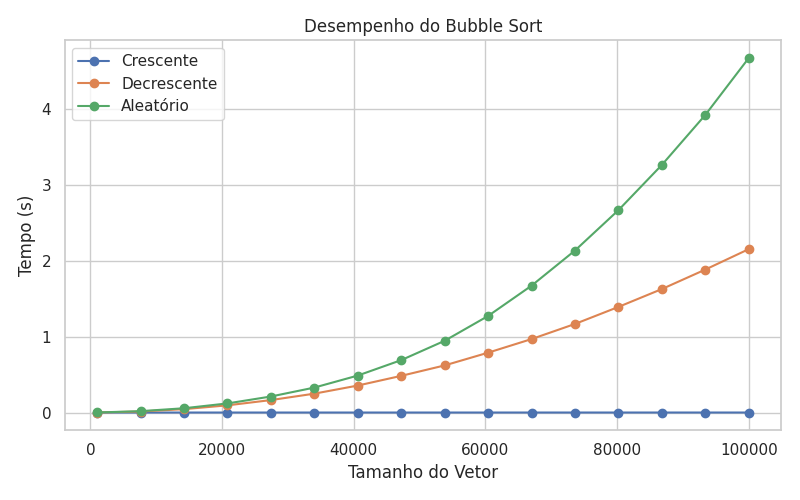
\includegraphics[width=1\textwidth]{../codigos/resultados/bubble_grafico.png}
    \caption{Tempo de execução do Bubble Sort para diferentes entradas}
    \label{fig:bubble-grafico}
\end{figure}

\subsection{Insertion Sort}
\begin{lstlisting}[language=C, caption={Implementação do Insertion Sort}, label={lst:insertion}]
void insertion_sort(int *v, int len)
{
    register int i, j;
    for(i=1; i<len; i++)
    {
        int key = v[i];
        for(j=i-1; j>=0 && v[j]>key; j--)
            v[j+1] = v[j];
        v[j+1] = key;
    }
}
\end{lstlisting}

\subsubsection{Complexidade Teórica}

O algoritmo \textit{Insertion Sort} percorre o vetor da esquerda para a direita, inserindo cada elemento na posição correta em relação aos anteriores. Ele é eficiente para vetores pequenos ou quase ordenados.

No pior caso, o vetor está ordenado em ordem decrescente. A cada nova iteração, o elemento atual precisa ser comparado com todos os anteriores, deslocando-os para a direita. Isso leva a:

\[
\sum_{i=1}^{n-1} i = \frac{n(n-1)}{2} = O(n^2)
\]

No melhor caso, quando o vetor já está em ordem crescente, nenhuma troca é feita — apenas uma comparação por iteração. Isso resulta em uma complexidade de tempo linear:

\[
O(n)
\]

No caso médio, assumindo entradas aleatórias, espera-se que cada elemento percorra metade dos anteriores, o que leva novamente a:

\[
O(n^2)
\]

A complexidade de espaço é \(O(1)\), pois o algoritmo é in-place e não utiliza estruturas auxiliares adicionais.~\cite{geeksforgeeks_insertion_sort}

\subsubsection{Resultados Experimentais}
\begin{figure}[H]
    \centering
    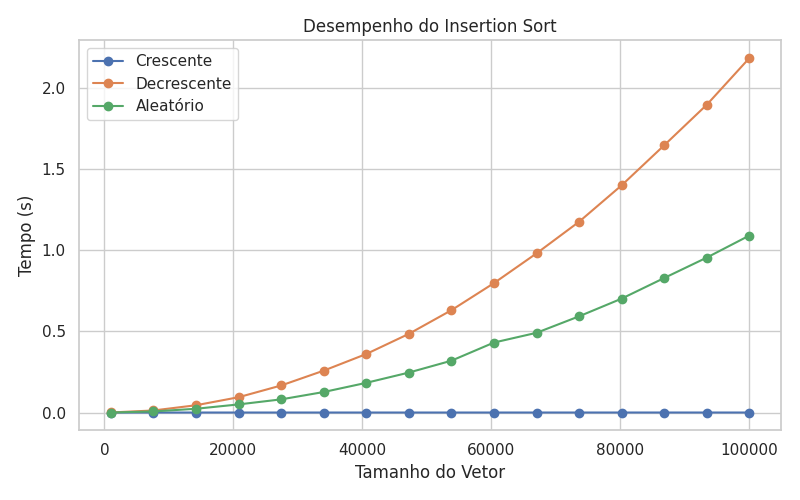
\includegraphics[width=1\textwidth]{../codigos/resultados/insertion_grafico.png}
    \caption{Tempo de execução do Insertion Sort para diferentes entradas}
    \label{fig:insertion-grafico}
\end{figure}

\subsection{Quick Sort}
\begin{lstlisting}[language=C, caption={Implementação do Quick Sort}, label={lst:quick}]
int lomuto(int *v, int low, int high)
{
    int *pivot = &v[high];
    int boundary = low;
    for(int i=low; i<high; i++) {
        if(v[i] <= *pivot)
            swap(&v[i], &v[boundary++]);
    }
    swap(pivot, &v[boundary]);

    return boundary;
}

int hoare(int *v, int low, int high)
{
    int i=low-1, j=high+1;
    int pivot = v[low];
    while(1) {
        do {
            i++;
        } while(v[i] < pivot);
        do {
            j--;
        } while(v[j] > pivot);
        if(i>=j)
            return j;
        swap(&v[i], &v[j]);
    }
}

void quick_sort(int *v, int low, int high)
{
    if(low < high) {
        int boundary = hoare(v, low, high);
        quick_sort(v, low, boundary);
        quick_sort(v, boundary+1, high);
    }
}
\end{lstlisting}

\subsubsection{Complexidade Teórica}

O \textit{Quick Sort} é um algoritmo baseado na estratégia de divisão e conquista. Ele escolhe um elemento pivô e reorganiza o vetor de forma que todos os elementos menores que o pivô fiquem à sua esquerda e os maiores à direita. Esse processo é repetido recursivamente em cada subvetor.

Existem duas estratégias principais de particionamento:

\begin{itemize}
    \item \textbf{Lomuto:} escolhe normalmente o último elemento como pivô. O particionamento é mais simples, mas menos eficiente em alguns casos devido ao maior número de trocas.
    
    \item \textbf{Hoare:} utiliza dois ponteiros que percorrem o vetor a partir das extremidades, trocando elementos fora de lugar. Costuma realizar menos trocas e é mais eficiente na prática.
\end{itemize}

A complexidade do Quick Sort depende da escolha do pivô:

\begin{itemize}
    \item \textbf{Melhor caso:} o pivô divide o vetor em duas partes iguais a cada recursão. Isso resulta em:
    \[
    O(n \log n)
    \]

    \item \textbf{Pior caso:} o pivô é sempre o menor ou o maior elemento, criando partições de tamanho \(n-1\) e 0. Isso leva a:
    \[
    O(n^2)
    \]

    \item \textbf{Caso médio:} em geral, o particionamento divide o vetor razoavelmente bem, levando a:
    \[
    O(n \log n)
    \]
\end{itemize}

O Quick Sort é um algoritmo in-place (com complexidade de espaço \(O(\log n)\) devido à recursão), e sua versão padrão
não é estável. Porém, por sua eficiência prática e uso frequente da memória cache, é amplamente utilizado.~\cite{geeksforgeeks_quick_sort}

\subsubsection{Resultados Experimentais}
\begin{figure}[H]
    \centering
    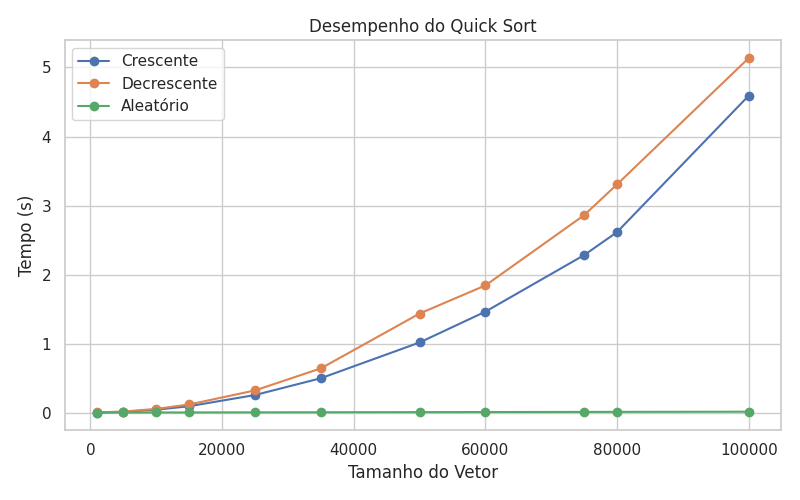
\includegraphics[width=1\textwidth]{../codigos/resultados/quick_grafico.png}
    \caption{Tempo de execução do Quick Sort com método de Hoare para diferentes entradas}
    \label{fig:quick_hoare-grafico}
\end{figure}

\subsection{Merge Sort}
\begin{lstlisting}[language=C, caption={Implementação do Merge Sort}, label={lst:merge}]
void merge(int v[], int low, int mid, int high)
{
    int n1 = mid-low+1;
    int n2 = high-mid;
    int v1[n1], v2[n2];

    for(int i=0; i<n1; i++)
        v1[i] = v[low+i];
    for(int i=0; i<n2; i++)
        v2[i] = v[mid+1+i];

    int i=0,j=0,k=low;
    while(i<n1 && j<n2)
    {
        if(v1[i] < v2[j])
            v[k++] = v1[i++];
        else
            v[k++] = v2[j++];
    }
    while(i<n1)
        v[k++] = v1[i++];
    while(j<n2)
        v[k++] = v2[j++];
}

void merge_sort(int *v, int low, int high)
{
    if(low < high) {
        int mid = (low+high)/2;
        merge_sort(v, low, mid);
        merge_sort(v, mid+1, high);

        merge(v, low, mid, high);
    }
}
\end{lstlisting}

\subsubsection{Complexidade Teórica}

O algoritmo \textit{Merge Sort} segue a estratégia de \textit{divisão e conquista}. Ele divide o vetor recursivamente ao meio até que cada subvetor tenha tamanho 1 e, em seguida, realiza a fusão (\textit{merge}) ordenada desses subvetores.

Em cada nível da recursão, o vetor é dividido pela metade, resultando em \(\log_2 n\) níveis. A cada nível, ocorre a fusão de todos os elementos, com custo proporcional a \(n\). Portanto, a complexidade no pior, melhor e caso médio é:

\[
O(n \log n)
\]

O desempenho do Merge Sort é estável, independentemente da ordem inicial dos dados, e ele sempre realiza o mesmo número de comparações e fusões.

Entretanto, como a fusão exige a criação de vetores auxiliares para armazenar temporariamente os dados, o Merge Sort não é in-place. Isso leva a uma complexidade de espaço adicional de:

\[
O(n)
\]

Apesar disso, sua eficiência e previsibilidade o tornam uma boa escolha para dados grandes e em aplicações que exigem
estabilidade na ordenação.~\cite{geeksforgeeks_merge_sort}

\subsubsection{Resultados Experimentais}
\begin{figure}[H]
    \centering
    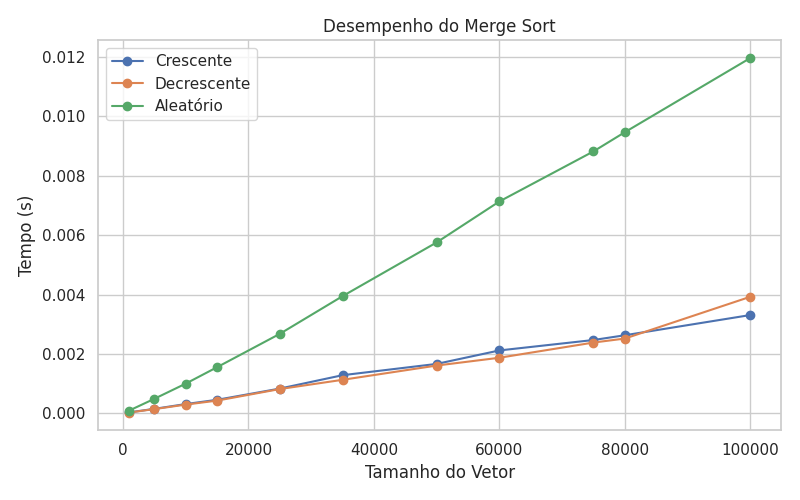
\includegraphics[width=1\textwidth]{../codigos/resultados/merge_grafico.png}
    \caption{Tempo de execução do Merge Sort para diferentes entradas}
    \label{fig:merge-grafico}
\end{figure}

\subsection{Heap Sort}
\begin{lstlisting}[language=C, caption={Implementação do Heap Sort}, label={lst:heap}]
void max_heapify(int v[], int n, int i)
{
    int l = 2*i+1;
    int r = 2*i+2;
    int larg = i;
    if(l < n && v[l] > v[larg])
        larg = l;
    if(r < n && v[r] > v[larg])
        larg = r;
    if(larg != i) {
        swap(&v[larg], &v[i]);
        max_heapify(v, n, larg);
    }
}

void heap_sort(int *v, int n)
{
    for(int i=n/2-1; i>=0; i--)
        max_heapify(v, n, i);

    n--;
    while(n) {
        swap(&v[0], &v[n--]);
        max_heapify(v, n, 0);
    }
}
\end{lstlisting}

\subsubsection{Complexidade Teórica}

O \textit{Heap Sort} é um algoritmo de ordenação baseado em uma estrutura de dados chamada \textit{heap}, que é uma árvore binária completa com a propriedade de heap (no caso do max-heap, cada nó é maior que seus filhos).

O algoritmo funciona em duas fases:

\begin{enumerate}
    \item Construção do heap a partir do vetor desordenado (fase de construção).
    \item Repetidamente extrair o maior elemento (raiz do heap) e reestruturar o heap restante (fase de ordenação).
\end{enumerate}

A análise da complexidade é dividida da seguinte forma:

\begin{itemize}
    \item \textbf{Construção do heap:} cada elemento é movido para manter a propriedade do heap, o que leva tempo proporcional à sua altura. No total, essa fase tem complexidade:
    \[
    O(n)
    \]

    \item \textbf{Remoção e reestruturação:} cada uma das \(n\) remoções exige uma operação de \textit{heapify}, com custo \(O(\log n)\), resultando em:
    \[
    O(n \log n)
    \]

    \item \textbf{Complexidade total:}
    \[
    O(n \log n)
    \]
\end{itemize}

O Heap Sort é um algoritmo in-place, pois utiliza apenas uma quantidade constante de memória adicional (\(O(1)\)). No
entanto, ele não é estável, e, embora sua complexidade seja semelhante à do Quick Sort no caso médio, tende a ser mais
lento em prática por causa do maior custo constante das operações de heap.~\cite{geeksforgeeks_heap_sort}

\subsubsection{Resultados Experimentais}
\begin{figure}[H]
    \centering
    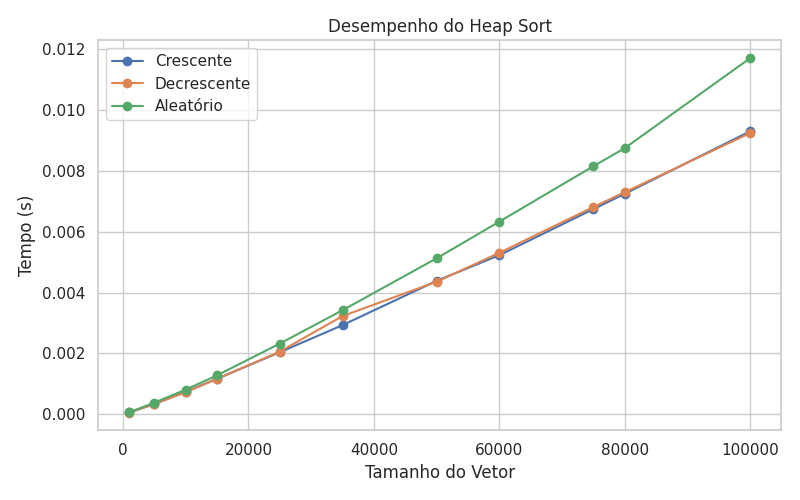
\includegraphics[width=1\textwidth]{../codigos/resultados/heap_grafico.png}
    \caption{Tempo de execução do Heap Sort para diferentes entradas}
    \label{fig:heap-grafico}
\end{figure}

\subsection{Radix Sort}
\begin{lstlisting}[language=C, caption={Implementação do Radix Sort}, label={lst:radix}]
int getmax(int v[], int len)
{
    int max = v[0];
    for(int i=1; i<len; i++)
        if(v[i]>max) max = v[i];
    return max;
}

void counting_sort(int v[], int len, int exp)
{
    int *answer = malloc(len * sizeof(int));
    int count[10] = {0};

    int i;
    for(i=0; i<len; i++)
        count[(v[i]/exp)%10]++;
    for(i=1; i<10; i++)
        count[i] += count[i-1];
    for(i=len-1; i>=0; i--) {
        answer[count[(v[i]/exp)%10]-1] = v[i];
        count[(v[i]/exp)%10]--;
    }
    for(i=0; i<len; i++)
        v[i] = answer[i];

    free(answer);
}

void radix_sort(int *v, int len)
{
    int max = getmax(v, len);

    for(int i=1; max/i>0; i*=10)
        counting_sort(v, len, i);
}
\end{lstlisting}

\subsubsection{Complexidade Teórica}

O \textit{Radix Sort} é um algoritmo de ordenação não-comparativo que ordena os elementos analisando seus dígitos, da menor posição (menos significativa) até a maior (mais significativa), utilizando um algoritmo de ordenação estável como sub-rotina (geralmente o \textit{Counting Sort}).

A ideia é ordenar os números várias vezes, uma para cada posição decimal, garantindo que ao final os números estejam
completamente ordenados.~\cite{geeksforgeeks_radix_sort}

\begin{itemize}
    \item Sejam:
    \begin{itemize}
        \item \(n\): o número de elementos a serem ordenados,
        \item \(k\): o maior valor presente no vetor,
        \item \(d\): o número de dígitos do maior elemento (em base 10).
    \end{itemize}
    
    \item Para cada dígito, o \textit{Counting Sort} é aplicado com tempo \(O(n + b)\), onde \(b\) é o tamanho da base (geralmente 10).
    
    \item Como o algoritmo realiza \(d\) passagens, a complexidade total será:
    \[
    O(d \cdot (n + b))
    \]

    \item Como \(d = \log_b(k)\), podemos reescrever como:
    \[
    O(n \cdot \log k)
    \]

    \item Assumindo que \(k\) é limitado por um inteiro de tamanho fixo (como 32 bits), o algoritmo pode ser considerado linear:
    \[
    O(n)
    \]
\end{itemize}

\textbf{Espaço:} O Radix Sort não é in-place, pois utiliza memória auxiliar proporcional ao tamanho da entrada e à base.

\textbf{Estabilidade:} O algoritmo é estável, desde que a sub-rotina de ordenação utilizada também o seja (como o Counting Sort).

\subsubsection{Resultados Experimentais}
\begin{figure}[H]
    \centering
    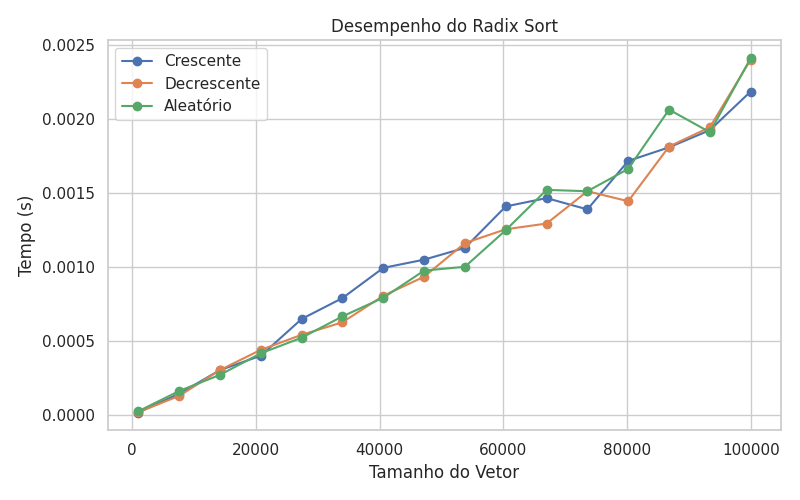
\includegraphics[width=1\textwidth]{../codigos/resultados/radix_grafico.png}
    \caption{Tempo de execução do Radix Sort para diferentes entradas}
    \label{fig:radix-grafico}
\end{figure}
